% Include the figure here so it goes to the top of the third page
\section{Locally Invariant Layer} \label{sec:ch5:method}
We propose to mix the terms at the output of each wavelet modulus propagator
$\widetilde{\mathcal{W}}$. The second term in $\widetilde{\mathcal{W}}$, the $U$
terms, are often called `covariant' terms but in this work, we will call them
\emph{locally invariant}, as they tend to be invariant up to a scale $2^j$. We propose
to mix these locally invariant terms $U$ and the lowpass terms $S$ with learned
weights $a_{f,\lambda}$ and $b_f$. 

For example, consider the wavelet modulus propagator from
\eqref{eq:ch5:wave_mod}, and let the input to it be $x^{(l)}$. Our proposed
output is then:
%
\begin{align} \label{eq:ch5:comb1}
  y^{(l+1)}(f, \xy)  &=  \sum_{\lambda\in \Lambda} \sum_{c=0}^{C-1} a_{f, \lambda}(c) \left|x^{(l)}(c, \xy)\conv \psi_\lambda(\xy)\right|
                     +  \sum_{c=0}^{C-1} b_f(c)\left(x^{(l)}(c, \xy) \conv \phi_J(\xy)\right) \\
                     &=\sum_{c=0}^{C-1} \left( b_f(c)\left(x^{(l)}(c, \xy) \conv \phi_J(\xy)\right) + 
                     \sum_{\lambda\in \Lambda} a_{f, \lambda}(c) \left|x^{(l)}(c, \xy)\conv \psi_\lambda(\xy)\right|\right) \label{eq:ch5:layer}
\end{align}

% Recall that $\lambda$ is the tuple $(j, k)$ for  $1 \leq j \leq J,\ 0 \leq k < K$
% and is used to select the bandpass wavelet at scale $j$ and orientation $k$.
Note that an input to the wavelet modulus propagator $\widetilde{\mathcal{W}}$ with $C$ channels
has $(JK+1)C$ output channels -- $C$ lowpass channels and $JKC$ modulus bandpass
channels. Let us define a new output $z$ with index variable $q\in \integers$ such that:
%
\begin{equation}
  z^{(l+1)}(q, \xy) =  \left\{
    \begin{array}{ll}
      x^{(l)}(c, \xy) \conv \phi_J(\xy) & \mbox{if } 0 \leq q < C \\
      |x^{(l)}(c, \xy)\conv \psi_\lambda(\xy)| & \mbox{if }	C \leq q < (JK+1)C
    \end{array}
    \right. \label{eq:ch5:z}
\end{equation}
i.e.\ the lowpass channels are the first $C$ channels of $z$, the modulus of the
$15\degs$ ($k=0$) wavelet coefficients with $j=1$ are the next $C$ channels,
then the modulus coefficients with $k=1$ and $j=1$ are the third $C$ channels,
and so on. This is similar to the view of a ScatterNet we introduced in \autoref{alg:ch3:dtcwt_scat},
but restricted to a single order.

We do the same for the weights $a,\ b$ by defining $\tilde{a}_f = \{b_f, a_{f,
\lambda} \}_{\lambda}$ and let:
\begin{equation}
  \tilde{a}_f(q) =  \left\{
    \begin{array}{ll}
      b_f(c) & \mbox{if } 0 \leq q < C \\
      a_{f, \lambda}(c) & \mbox{if }	C \leq q < (JK+1)C
    \end{array}
    \right. \label{eq:ch5:tilde_a}
\end{equation}
%
we can then use \eqref{eq:ch5:z} and \eqref{eq:ch5:tilde_a} to simplify 
\eqref{eq:ch5:layer}, giving:
\begin{equation}
  y^{(l+1)}(f, \xy)  =  \sum_{q=0}^{(JK + 1)C - 1} z^{(l+1)}(q, \xy) \tilde{a}_f(q) \label{eq:ch5:mixing}
\end{equation}
or in matrix form with $A_{f,q} = \tilde{a}_f(q)$
%
\begin{equation}
  Y^{(l+1)}(\xy)  =  A Z^{(l+1)}(\xy) \label{eq:ch5:matrix}
\end{equation}

This equation now looks very similar to the standard convolutional layer from
\eqref{eq:ch5:conv}, except we have replaced the previous layer's $x$ with
intermediate coefficients $z$ with $|Q| = (JK+1)C$ channels and the
convolutions of \eqref{eq:ch5:conv} have been replaced by a matrix multiply
(which can also be seen as a $1\x 1$ convolutional layer). We can then apply
\eqref{eq:ch5:nonlin} to \eqref{eq:ch5:mixing} to get the next layer's output:
%
\begin{equation}
  x^{(l+1)}(f, \xy) = \sigma\left( y^{(l+1)}(f, \xy) \right)
  \label{eq:ch5:xnext}
\end{equation}
\autoref{fig:ch5:block_diagram} shows a block diagram for this process. 

\begin{figure}[t!]
  \centering
  % \small
  % \resizebox{\textwidth}{!} {
    % \begin{tikzpicture}[%
  path image/.style={
    path picture={
      \node at (path picture bounding box.center) {
        \includegraphics[height=2.0cm]{#1}
      };
    }
  }, 
  path pic/.style={
    path picture={
      \node at (path picture bounding box.center) {
        \includegraphics[height=1.2cm]{#1}
      };
    }
  }, 
  path pic2/.style={
    path picture={
      \node at (path picture bounding box.center) {
        \includegraphics[height=0.8cm]{#1}
      };
    }
  }, 
  scale=0.6]

  \tikzcuboid{
  shiftx=-1.5cm,
  shifty=-2.5cm,
  scale=0.5,
  anglex=0, 
  angley=90, 
  anglez=230,
  dimx=3, 
  dimy=3, 
  dimz=6,
  densityx=1, 
  densityy=1, 
  densityz=1,
  shade=false,
  emphedge=true,
  shadeopacity=0,
  emphstyle/.style={rounded corners=0.2pt,line width=0.3mm},
  front/.style={draw=blue!50!white,fill=blue!50!white},%
  right/.style={draw=blue!50!white,fill=blue!50!white},%
  top/.style={draw=blue!50!white,fill=blue!50!white},%
  drawxdims=true,
  dimxval=W,
  drawydims=true,
  dimyval=H,
  drawzdims=true,
  dimzval=C_l,
  }
  \draw (0, .3, 0) node {\large{$x^{(l)}$}};
  \draw [path image=\imgpath/waveys.png, draw=black] (1.5,1.5,0) rectangle (6,0,0);
  \draw (3.75, 1.9, 0) node {\large{$\psi_{j, \theta}$}};
  \draw (1.5,0,0) -- (3,-1.7,0);
  \draw (6,0,0) -- (3.3,-1.7,0);
  \draw [path pic2=\imgpath/lowpass.png, draw=black] (2.5,-2.5,10) rectangle (3.5,-1.5,10);
  \draw (3, -1.1, 10) node {\large{$\phi_{j}$}};
  \draw (3.5,-1.5,10) -- (3.5,-1.7,8);

  % \draw (2.4, -1.5, 0) node {\Large{$\conv$}};
  \draw (2.5, -1.5, 3) node {\Large{$\conv$}};
  \draw [->, fill=gray!30,ultra thick] (4, -1.5, 0) -- (5, -1.5, 0);
  \draw [->, fill=gray!30,ultra thick] (4.5, -1.5, 9) -- (5.85, -1.5, 11);

  \tikzcuboid{
  shiftx=3cm,
  shifty=-1.7cm,
  shiftz=0,
  scale=0.3,
  dimx=1, dimy=1, dimz=4,
  densityx=2, densityy=2, densityz=2,
  drawxdims=false,
  drawydims=false,
  drawzdims=true,
  dimzval=12,
  front/.style={draw=yellow!70!white,fill=yellow!70!white},%
  right/.style={draw=yellow!70!white,fill=yellow!70!white},%
  top/.style={draw=yellow!70!white,fill=yellow!70!white},%
  }
  \tikzcuboid{
  shiftz=8/0.3,
  scale=0.3,
  dimx=1, dimy=1, dimz=1,
  densityx=2, densityy=2, densityz=2,
  drawxdims=false,
  drawydims=false,
  drawzdims=false,
  }


  \tikzcuboid{
  shiftx=6cm,
  shifty=-2.0cm,
  shiftz=0.8cm,
  scale=0.5,
  dimx=2, dimy=2, dimz=4,
  densityx=4, densityy=4, densityz=2,
  drawzdims=true,
  dimzval=C_l,
  front/.style={draw=blue!50!white,fill=blue!50!white},%
  right/.style={draw=blue!50!white,fill=blue!50!white},%
  top/.style={draw=blue!50!white,fill=blue!50!white},%
  }

  \tikzcuboid{
  shiftx=6cm,
  shifty=-2cm,
  shiftz=0cm,
  scale=0.5,
  dimx=2, dimy=2, dimz=24,
  densityx=2, densityy=2, densityz=2,
  drawxdims=true,
  dimxval=\frac{W}{2},
  drawydims=true,
  dimyval=\frac{H}{2},
  drawzdims=true,
  dimzval=12C_l,
  front/.style={draw=blue!50!white,fill=blue!50!white},%
  right/.style={draw=blue!50!white,fill=blue!50!white},%
  top/.style={draw=blue!50!white,fill=blue!50!white},%
  }

  % \draw [->, fill=gray!30,ultra thick] (8.5, -1.5, 0) -- (10.5, -1.5, 0) node[midway, above] (mag) {\large{$\lvert\cdot\rvert$}};
  \draw [->, fill=gray!30,ultra thick] (8.5, -1.5, 0) -- (10.5, -1.5, 0) node[midway, above] (mag) {\Large{ $\lvert \cdot \rvert$} };
  \draw [path pic=\imgpath/mag.png, draw=white] (9.25,0,0) rectangle (11.75,2,0);
  \draw (9.25,0,0) -- (mag.north);
  \draw (11.75,0,0) -- (mag.north);
  \draw[->, fill=gray!30, ultra thick] (8.5, -2, 10) -- (10, -3, 3);

  \tikzcuboid{
  shiftx=11.5cm,
  shifty=-2cm,
  scale=0.5,
  dimx=2, dimy=2, dimz=12,
  densityx=2, densityy=2, densityz=2,
  dimzval=6C_l,
  drawxdims=false,
  drawydims=false,
  front/.style={draw=blue!50!white,fill=blue!50!white},%
  right/.style={draw=blue!50!white,fill=blue!50!white},%
  top/.style={draw=blue!50!white,fill=blue!50!white},%
  }
  \tikzcuboid{
  shiftx=11.5cm,
  shifty=-2cm,
  shiftz=8,
  scale=0.5,
  drawxdims=true,
  drawydims=true,
  dimx=2, dimy=2, dimz=4,
  densityx=2, densityy=2, densityz=2,
  dimzval=C_l,
  front/.style={draw=blue!50!white,fill=blue!50!white},%
  right/.style={draw=blue!50!white,fill=blue!50!white},%
  top/.style={draw=blue!50!white,fill=blue!50!white},%
  }
  \draw (13.2, 0.8, 0) node {\large{$z^{(l+1)}$}};
  \draw (20.5, 0.3, 0) node {\large{$y^{(l+1)}$}};
  \draw (24.5, 0.3, 0) node {\large{$x^{(l+1)}$}};
  \draw (14, -1.5, 0) node {\Large{$\conv$}};

  \tikzcuboid{
  shiftx=15.2cm,
  shifty=-1.0cm,
  shiftz=0,
  scale=0.5,
  dimx=0.4, dimy=0.4, dimz=14,
  densityx=5, densityy=5, densityz=2,
  drawxdims=false,
  drawydims=false,
  drawzdims=false,
  front/.style={draw=red!50!white,fill=red!50!white},%
  right/.style={draw=red!50!white,fill=red!50!white},%
  top/.style={draw=red!50!white,fill=red!50!white},%
  }
  \tikzcuboid{
  shifty=-1.65cm,
  }
  \tikzcuboid{
  shifty=-3.0cm,
  scale=0.5,
  drawxdims=true,
  dimxval=1,
  drawydims=true,
  dimyval=1,
  drawzdims=true,
  dimzval=7C_l,
  }
  \draw (15.5, -1.8, 0) node {$\vdots$};
  \draw [<->] (15.7, -0.8, -3) -- (15.7, -3, -3) node[near start, right] {$C_{l+1}$};
  \draw [->, fill=gray!30,ultra thick] (17.5, -1.5, 0) -- (18.5, -1.5, 0);

  \tikzcuboid{
  shiftx=19.5cm,
  shifty=-2.25cm,
  scale=0.5,
  dimx=2, dimy=2, dimz=6,
  densityx=4, densityy=4, densityz=2,
  drawzdims=false,
  drawxdims=false,
  drawydims=false,
  front/.style={draw=blue!50!white,fill=blue!50!white},%
  right/.style={draw=blue!50!white,fill=blue!50!white},%
  top/.style={draw=blue!50!white,fill=blue!50!white},%
  }
  \draw [->, fill=gray!30,ultra thick] (21.5, -1.5, 0) -- (22.5, -1.5, 0)
    node[midway, above] {$\sigma$};

  \tikzcuboid{
  shiftx=23.5cm,
  shifty=-2.25cm,
  scale=0.5,
  dimx=2, dimy=2, dimz=6,
  densityx=4, densityy=4, densityz=2,
  drawzdims=true,
  dimzval=C_{l+1},
  drawxdims=true,
  dimxval=\frac{W}{2},
  drawydims=true,
  dimyval=\frac{H}{2},
  front/.style={draw=blue!50!white,fill=blue!50!white},%
  right/.style={draw=blue!50!white,fill=blue!50!white},%
  top/.style={draw=blue!50!white,fill=blue!50!white},%
  }

\end{tikzpicture}

 
  % }
  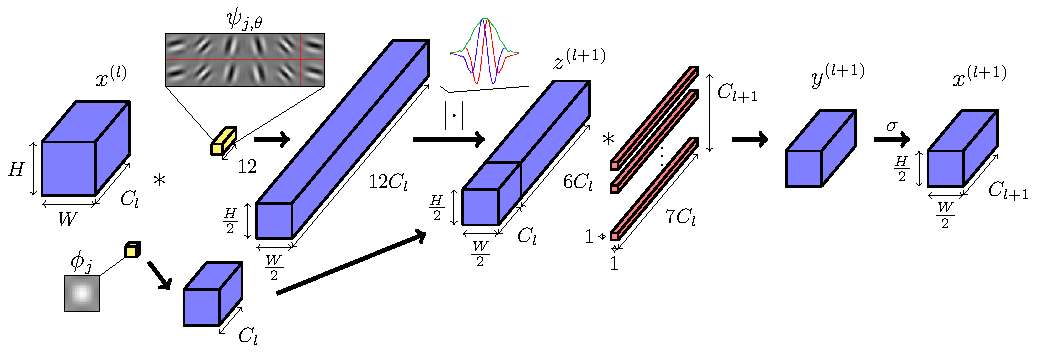
\includegraphics[width=\textwidth]{\imgpath/figure1.pdf}
  \mycaption{Block Diagram of Proposed Invariant Layer for $j=J=1$}{Activations are shaded
  blue, fixed parameters yellow and learned parameters red. Input
  $x^{(l)}\in \mathbb{R}^{C_l\x H\x W}$ is filtered by real and imaginary oriented
  wavelets and a lowpass filter and is downsampled. The channel dimension
  increases from $C_l$ to $(2K+1)C_l$, where the number of orientations is $K=6$.
  The real and imaginary parts are combined by taking their magnitude (an
  example of what this looks like in 1D is shown above the magnitude operator) -
  taking the envelope of the components oscillating in quadrature. These are 
  concatenated with the lowpass activations to give $z^{(l+1)}$. The
  resulting activations $z$ are mixed across the channel dimension and then passed through a nonlinearity
  $\sigma$ to give $x^{(l+1)}$. If the desired output spatial size is $H\x W$,
  $x^{(l+1)}$ can be bilinearly upsampled paying only a few multiplies per
  pixel.}
  \label{fig:ch5:block_diagram}
\end{figure}

\subsection{Properties}
\subsubsection{Recovering the original ScatterNet Design}
The first thing to note is that with careful choice of $A$ and $\sigma$, we can
recover the original translation-invariant ScatterNet
\cite{bruna_invariant_2013, oyallon_scaling_2017}. If $C_{l+1} = (JK+1)C_l$ 
and $A$ is the identity matrix $I_{C_{l+1}}$, there is no mixing and $y^{(l+1)} = \widetilde{\mathcal{W}}x$.

Further, if $\sigma = \F{ReLU}$ as is commonly the case in training CNNs,
$\sigma$ has no effect on the positive locally invariant terms $U$. It will affect the averaging terms
if the signal is not positive, but this can be dealt with by adding a channel-dependent 
bias term $\alpha_c$ to $x^{(l)}$ to ensure it is positive. This bias term
will not affect the propagated signals as $\int \alpha_c \psi_\lambda(\xy) d\xy =
0$. The bias can then be corrected by subtracting $\alpha_c \norm{\phi_J}_2$ from
the averaging terms after taking the ReLU, then $x^{(l+1)} =
\widetilde{\mathcal{W}}x$.

This makes one layer of our system equivalent to a first-order scattering
transform, giving $S_0$ and $U_1$ (invariant to input shifts of $2^1$). We can repeat
the same process for the next layer (recall the recursive scattering relation we
saw in \eqref{eq:ch2:recursive}),
giving $S_1$ and $U_2$ (invariant to shifts of $2^2$). If we want to build
higher invariance, we can continue or simply average these outputs with an average pooling
layer.

\subsubsection{Flexibility of the Layer}
Unlike a regular ScatterNet, we are free to choose the size of $C_{l+1}$. This
means we can set $C_{l+1} = C_{l}$ as is commonly the case in a CNN, and make a
convolutional layer from mixing the locally invariant terms. This avoids the
exponentially increasing complexity that comes with extra network layers that 
standard ScatterNets suffer from.

\subsubsection{Stability to Noise and Deformations}
Let us define the action of our layer on the scattering
coefficients to be $Vx$. We would like to find a bound on $\norm{V\mathcal{L}_\tau x -
V x}$. To do this, we note that the mixing is a linear operator and hence is
Lipschitz continuous. The authors in \cite{qiu_dcfnet:_2018} find constraints on the mixing
weights to make them non-expansive (i.e. Lipschitz constant 1).
Further, the ReLU is non-expansive meaning the combination of the two is
also non-expansive, so $\norm{V\mathcal{L}_\tau x - V x} \leq \norm{S\mathcal{L}_\tau
x - Sx}$, and \eqref{eq:ch2:stability} holds.
% We would also like to ensure that we can derive a similar bound in stability to
% \eqref{eq:ch5:stability}. Let us call the action of our layer (with learned
% weights and nonlinearity) $Vx = \sigma(M[\gamma]\tilde{W}[\gamma]x)$. We would like to find a bound on
% $\norm{V\mathcal{L}_\tau x - V x}$. Fortunately, $M[\gamma]$ is a linear
% operator, so it is not difficult to find constraints on it that make it
% non-expansive. Proposition 3.1 in \autoref{qiu_dcfnet:ch5:_2018} does just this for
% the ReLU and convolutional layer

% \begin{eqnarray}
% \norm{V\mathcal{L}_\tau x - V x} = 
% \end{eqnarray}

